\definecolor{customred}{HTML}{E7180B}

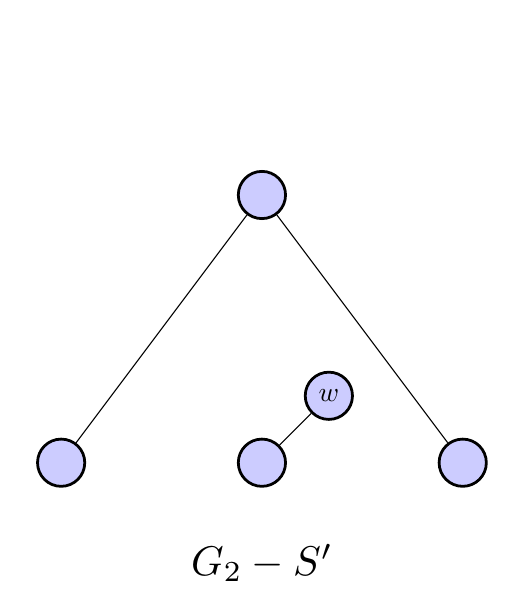
\begin{tikzpicture}[scale=0.85, auto=left]
  \tikzset{
    blue_node/.style={circle, fill=blue!20, draw, line width=1pt, inner sep=2pt, minimum size=6mm},
    red_node/.style={circle, fill=customred!20, draw=customred, line width=1pt, inner sep=2pt, minimum size=6mm}
  }

  % Vértices según la cuadrícula
  % Vértices con etiqueta
  \node[blue_node] (v) at (3,2) [opacity=0]{$v$};
  \node[blue_node] (u) at (2,1) [opacity=0]{$u$};
  \node[blue_node] (w) at (4,1) {$w$};

  % Vértices sin etiqueta (círculos vacíos)
  \node[blue_node] (top) at (3,4) {};
  \node[blue_node] (bottom) at (3,0) {};
  \node[blue_node] (left_bottom) at (0,0) {};
  \node[blue_node] (right_bottom) at (6,0) {};

  % Aristas del diamante interno (u, v, w, bottom)

  % Conexiones del vértice superior (top)
  \draw (top) -- (left_bottom);
  \draw (top) -- (right_bottom);
  \draw (w) -- (bottom);
  % Conexión del vértice inferior izquierdo

  % Bounding box para asegurar la alineación de la figura
  \useasboundingbox (-0.5,-1.6) rectangle (6.5,6.5);

  % Etiqueta del grafo
  \node[draw=none, fill=none, scale=1.5] at (3,-1.5) {$G_2-S'$};
\end{tikzpicture}
